\section{Simulações}

\subsection{Métodos computacionais}

\lipsum[2-4]

\subsection{Resultados}

\begin{figure}[ht]
	\centering
	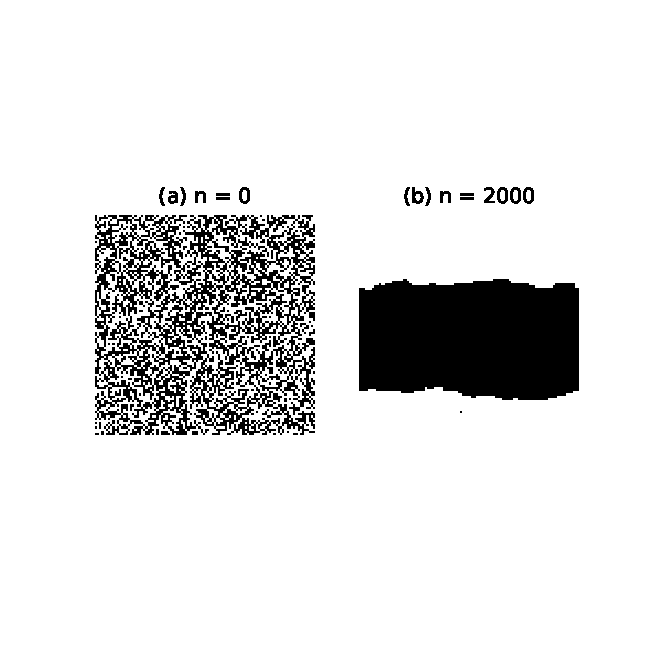
\includegraphics[scale = 1]{./img/evolucao-grid-100x100}
    \caption{Configurações inicial (esquerda) e final (direita) de um grid com $100 \times 100$ spins com condições periódicas de contorno e $J = 1$, $h = 0$ e $T/k_B = 1$. Para este exemplo, foram realizados $2000$ passos de Monte Carlo no algoritmo de Metropolis. O sistema é iniciado com uma configuração de spins aleatória e atinge um estado final com regiões compactas de mesma magnetização.}
    \label{fig:evolucao-grid-100x100}
\end{figure}

\begin{figure}[ht]
	\centering
	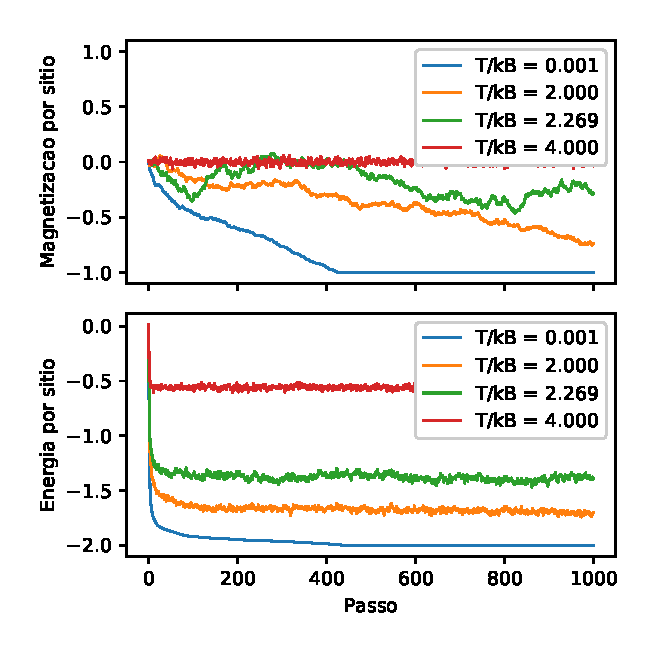
\includegraphics[scale = 1]{./img/evolucao-mc-temperaturas}
    \caption{Evolução da magnetização por sítio (acima) e da energia por sítio (abaixo) de um grid com $100 \times 100$ spins com condições periódicas de contorno e $J = 1$ e $h = 0$, a cada passo de Monte Carlo, para alguns valores de temperatura próximos à temperatura crítica (eq).}
    \label{fig:evolucao-mc-temperaturas}
\end{figure}

\begin{figure}[ht]
	\centering
	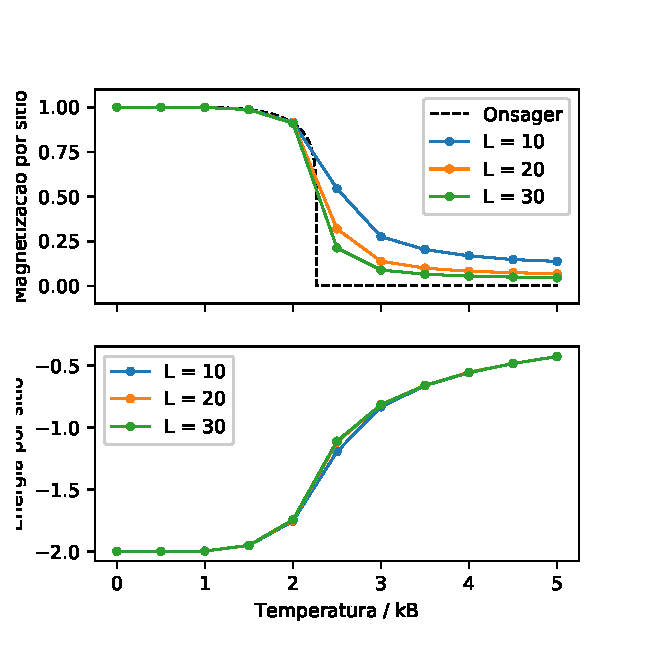
\includegraphics[scale = 1]{./img/simulacao-3-larguras}
    \caption{Curvas de magnetização por sítio (acima) e energia por sítio (abaixo) em função da temperatura de grids com $10 \times 10$, $20 \times 20$ e $30 \times 30$ spins com condições periódicas de contorno e $J = 1$ e $h = 0$.}
    \label{fig:simulacao-3-larguras}
\end{figure}

\begin{figure}[ht]
	\centering
	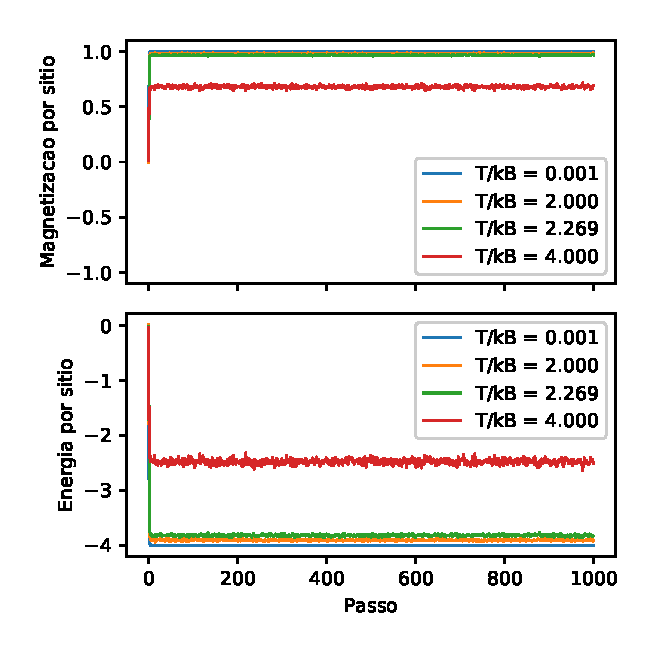
\includegraphics[scale = 1]{./img/evolucao-h=1-mc-temperaturas}
    \caption{Evolução da magnetização por sítio (acima) e da energia por sítio (abaixo) de um grid com $100 \times 100$ spins com condições periódicas de contorno e $J = 1$ e $h = 1$, a cada passo de Monte Carlo, para alguns valores de temperatura próximos à temperatura crítica (eq).}
    \label{fig:evolucao-h=1-mc-temperaturas}
\end{figure}

\begin{figure}[ht]
	\centering
	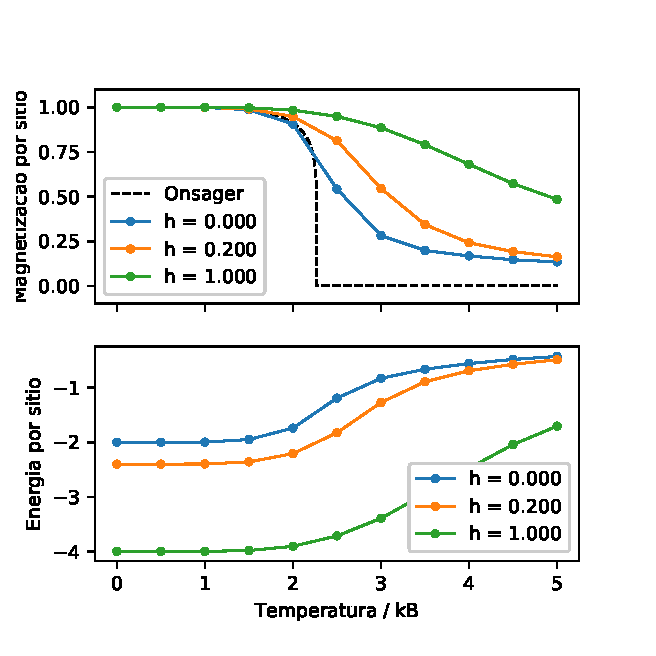
\includegraphics[scale = 1]{./img/simulacao-h}
    \caption{Curvas de magnetização por sítio (acima) e energia por sítio (abaixo) em função da temperatura de um grid com $10 \times 10$ spins com condições periódicas de contorno e $J = 1$ e $h = 0$, $0.2$ e $1$.}
    \label{fig:simulacao-h}
\end{figure}